\documentclass[a4paper,10pt]{article}
\setlength{\columnseprule}{0.1pt}
\setlength{\columnsep}{1cm}
\usepackage{CommandsAndStyle}

\author{Idea originaria di Federico Glaudo e Giada Franz \\
  Piccole aggiunte di Dario Balboni \\
  Contributo Fisico di Federico Franceschini}
\title{Formulario di Fisica II}

\begin{document}
\maketitle

\begin{multicols}{2}
\section{Costanti fisiche}
\formula{Costante dielettrica nel vuoto}{
  \begin{equation*}
    \ez=8.854\cdot 10^{-12}\frac Fm
  \end{equation*}
  \begin{equation*}
    k=\frac 1{4\pi\ez}=8.987 \cdot 10^9
  \end{equation*}
}
\formula{Permeabilità magnetica nel vuoto}{
  \begin{equation*}
    \muz=4\pi\cdot 10^{-7}=1.256 \cdot 10^{-6} \frac Hm
  \end{equation*}
}

\formula{Velocità della luce nel vuoto}{
  \begin{equation*}
    c=2.997\cdot 10^8\frac ms=\frac 1{\sqrt{\muz\ez}}
  \end{equation*}
}

\section{Leggi fondamentali del campo elettrico}
\formula{Legge di Coulomb}{
  Chiamando $\epsilon=\ez$ se siamo nel vuoto e $\epsilon=\ez\epsilon_r$ se siamo in un mezzo:
  \begin{equation*}
    \vec F=\frac 1{4\pi\epsilon}\frac{q_1q_2}{r^2}\hat r
  \end{equation*}
}

\formula{Campo elettrico}{
  \begin{equation*}
    \vec E(\vec r)=\frac 1{4\pi\ez}\int \rho(\vec r')\frac{\vec r-\vec r'}{\abs{\vec r-\vec r'}^3}\de \vec r'
  \end{equation*}
}

\formula{Potenziale}{
  \begin{equation*}
    V(\vec r)=\frac 1{4\pi\ez}\int \frac{\rho(\vec r')}{\abs{\vec r-\vec r'}}\de \vec r' 
  \end{equation*}
  
  \begin{equation*}
    \vec E=-\grad V
  \end{equation*}
}

\formula{Legge di Gauss}{
  \begin{equation*}
    \frac{Q_{int}}{\ez}=\frac 1\ez\int_\Omega \rho =\int_{\partial \Omega}\vec E\cdot \hat n
  \end{equation*}
}

\formula{I equazione di Maxwell}{
  \begin{equation*}
    \div \vec E=\frac\rho\ez
  \end{equation*}
}

\formula{II equazione di Maxwell (Elettrostatica)}{
  \begin{equation*}
    \rot \vec E=0
  \end{equation*}
}

\formula{Equazione di Poisson}{
  \begin{equation*}
    \lapl V=-\frac \rho \ez
  \end{equation*}
}

\formula{Energia elettrostatica}{
  \begin{equation*}
    U_E=\frac 12\int \int \frac 1{4\pi\ez}\cdot\frac{\rho(\vec r)\rho(\vec r')}{\abs{\vec r-\vec r'}}=\frac 12\int\rho V=\frac \ez 2\int \vec E^2 
  \end{equation*}
}

\formula{Forza agente su una carica}{
  La forza di Lorentz agente su una carica {\bf in assenza di campo magnetico} è
  \begin{equation*}
    \vec F = q \vec E
  \end{equation*}
}

\section{Primi termini dello sviluppo del potenziale}
Nel caso in cui la distribuzione di carica sia sufficientemente localizzata, si può sviluppare il potenziale ai primi ordini con le formule:
\formula{Termine di monopolo}{
  \begin{equation*}
    V(\vec r)\approx\frac 1{4\pi\ez r}\left(\int \rho\right)
  \end{equation*}
}
\formula{Termine di dipolo}{
  \begin{equation*}
    V(\vec r)\approx\frac {\vec r}{4\pi\ez r^3}\cdot\left(\int \rho\left(\vec r'\right)\vec r'\de \vec r'\right)
  \end{equation*}
}

\formula{Potenziale a simmetria cilindrica}{
  Attenzione che la formula seguente è scritta in coordinate sferiche e non in cilindriche: $r$ è il raggio e $\theta$ è l'angolo azimutale (quello che non fa un giro intero)

  \begin{equation*}
    V(r, \theta) = \sum_{l=0}^\infty \lrb{\frac{A_l}{r^{l+1}} + B_l r^l} P_l(\cos \theta)
  \end{equation*}

  I $P_l(\cos \theta)$ sono polinomi e si chiamano ``di Legendre''. Sono tra loro ortogonali, $\deg P_l = l$ e normalizzati in modo che $P_l(1) = 1$. I primi sono: $P_0(x) = 1, P_1(x) = x, P_2(x) = \frac{3x^2 - 1}{2}$
}

\section{Conduttori}

\formula{Pressione elettrostatica}{
  \begin{equation*}
    p=\frac{\de F^\perp}{\de S}=\frac{\de q}{\de S} \cdot\frac{E^\perp_{in}+E^\perp_{out}}2=\sigma \cdot\frac{E^\perp_{in}+E^\perp_{out}}2
  \end{equation*}
}

\formula{Campo e pressione sulla superficie di un conduttore}{
  \begin{equation*}
    E^\perp=\frac \sigma\ez
  \end{equation*}
  \begin{equation*}
    p=\sigma\frac {E^\perp}2=\frac{\sigma^2}{2\ez}
  \end{equation*}
  
}

\formula{Sistema di conduttori}{
  Chiamiamo $\vec Q=(Q_1,\dots,Q_n)$ il vettore delle cariche e $\vec V=(V_1,\dots,V_n)$ il vettore dei potenziali degli $n$ conduttori, allora esiste una matrice $C$ tale che $\vec Q=C\vec V$. Inoltre:
  \begin{equation*}
    U=\frac 12\sum Q_iV_i
  \end{equation*}
}
\end{multicols}

\section{Configurazioni speciali di carica}
% TODO: Scrivere anche l'energia elettrostatica per tutte le configurazioni
\formula{Campi e potenziali particolari}{
  \begin{description}
  \item[Carica puntiforme]
    \begin{equation*}
      \vec E(r)=\frac1{4\pi\ez}\cdot \frac Q{r^2}
    \end{equation*}
    \begin{equation*}
      V(r)=\frac1{4\pi\ez}\cdot \frac Qr
    \end{equation*}
    Non se ne può calcolare l'energia elettrostatica poiché diverge. I fisici la chiamano autoenergia e viene
    solitamente tolta negli altri conti per trovare l'energia elettrostatica.
    
  \item[Filo]\begin{equation*}
      \vec E(r)=\frac 1{2\pi\ez}\cdot\frac \lambda r
    \end{equation*}
    \begin{equation*}
      V(r)=-\frac\lambda{2\pi\ez}\ln(r)
    \end{equation*}
    
  \item[Piano]\begin{equation*}
      \vec E=\frac \sigma{2\ez}
    \end{equation*}
    \begin{equation*}
      V(r)=-\frac{\sigma r}{2\ez}
    \end{equation*}

  \item[Sfera uniformemente carica]
    Si suppone, ovviamente che $R$ sia il raggio della sfera, $Q = \frac{4}{3} \pi R^3 \rho$ la sua carica totale.
    \begin{equation*}
      \vec E(r) = \left\{ \begin{array}{lr}
                            \qpeo \frac{Q}{R^2} \frac{r}{R} \hat{r}
                            & \text{ dentro alla sfera } \\
                            \qpeo \frac{Q}{r^2} \hat{r}
                            & \text{ fuori dalla sfera } \\
                          \end{array} \right.
    \end{equation*}
    \begin{equation*}
      V(r) = \left\{ \begin{array}{lr}
                       \qpeo Q \left( - \frac{r^2}{2 R^3} + \frac{3}{2 R} \right)
                       & \text{ dentro alla sfera } \\
                       \qpeo \frac{Q}{r}
                       & \text{ fuori dalla sfera } \\
                     \end{array} \right.
    \end{equation*}
    \begin{equation*}
      U_E = \qpeo \frac{Q^2}{R} \frac{6}{5}
    \end{equation*}

  \item[Guscio sferico con carica superficiale] %TODO

  \item[Filo ciccione] %TODO
    
  \item[Due cariche uguali a distanza fissata]
    Si suppone che vi siano due cariche $Q$ (dello stesso valore e segno) a distanza $2D$. Useremo le coordinate
    cilindriche $\rho, z, \phi$.
    \vskip 0.5em
    \begin{tabular}{cc}
      $\vec E(z, \rho) = \qpeo \frac{2 Q}{(\rho^2 + (z - D)^2)(\rho^2 + (z + D)^2)} (z(\rho^2 + z^2 - D^2) \hat{z} + \rho
      (\rho^2 + z^2 + D^2) \hat{\rho})$
      & % TODO inserire il potenziale
    \end{tabular}

  \item[Due cariche diverse a distanza fissata] %TODO
  \end{description}
}

\begin{multicols}{2}

\formula{Dipolo}{
  \begin{equation*}
    V(\vec r)=\frac 1{4\pi\ez}\cdot \frac{\vec p\dotp \vec r}{r^3}
  \end{equation*}
  \begin{equation*}
    \vec E(\vec r)=\frac 1{4\pi\ez}\left(\frac{3(\vec p\dotp \hat r)\hat r-\vec p}{r^3} \right)
  \end{equation*}
  \begin{equation*}
    \tau=\vec p\times \vec E
  \end{equation*}
  \begin{equation*}
    \vec F=\Diff \vec E\dotp \vec p
  \end{equation*}

  \formula{Energia di un dipolo elettrico in un campo}{
    \begin{equation*}
      U = - \vec p \cdot \vec E (\vec r)    
    \end{equation*}
  }
  
  \formula{Momento forze del dipolo}{
    \begin{equation*}
      \vec M = \vec p \times \vec E
    \end{equation*}
  }
  
}

% TODO: formula quadrupolo

\formula{Carica immagine}{
  \begin{description}
  \item [Piano] Nel simmetrico rispetto al piano una carica $-q$.
  \item [Sfera a terra] Nell'inverso rispetto alla sfera, cioè in $x'=\frac{R^2}{x}$, una carica $q'=-\frac{qR}x$.
  \item [Sfera isolata] Se c'è una carica $q$ all'esterno della sfera, le cariche immagine (per risolvere il problema all'esterno della sfera) sono due: una nell'inverso rispetto alla sfera di carica $q'=-\frac{qR}x$ e una nel centro della sfera di carica $-q'$ (in modo che la carica totale nella sfera sia 0).
  \end{description}
}

\section{Condensatori}
\formula{Relazione tra carica e capacità}{
  \begin{equation*}
    Q = CV
  \end{equation*}
}

\formula{Relazione tra corrente e tensione}{
  \begin{equation*}
    I = C \ded{V}{t}
  \end{equation*}
}
  
\formula{Energia di un condensatore}{
  \begin{equation*}
    U=\frac 12QV=\frac 12CV^2=\frac12\frac {Q^2}C
  \end{equation*}
}

\formula{Capacità di vari condensatori}{
  Nota: la presenza di un materiale fra le armature di un condensatore ne aumenta la capacità di un fattore $\epsilon_r$ (numero puro) detto costante
  dielettrica relativa che dipende dalle caratteristiche del materiale. (Tutte le formule della capacità vengono moltiplicate per $\epsilon_r$)
  \begin{description}
  \item[Condensatore piano] \begin{equation*} 
      C=\frac{\ez S}d
    \end{equation*}
    dove $S$ è la superficie del condesatore e $d$ è la distanza fra le due piastre.
  \item[Condensatore cilindrico] \begin{equation*}
      C=\frac{2\pi\ez h}{\ln(\frac Rr)}
    \end{equation*}
    dove $h$ è l'altezza del cilindro e $R,r$ sono rispettivamente il raggio della piastra esterna e quello della piastra interna.
  \item[Condensatore sferico] \begin{equation*}
      C=4\pi\ez\frac{Rr}{R-r}
    \end{equation*}
    dove $R$ ed $r$ sono rispettivamente il raggio della piastra esterna e quello della piastra interna.
  \item[Conduttore sferico isolato] \begin{equation*}
      C=4\pi\ez r
    \end{equation*}
    
  \item[Condensatori in parallelo] \begin{equation*}
      C_{eq}=C_1+C_2
    \end{equation*}
  \item[Condensatori in serie]\begin{equation*}
      C_{eq}=\frac 1{\frac 1{C_1}+\frac 1{C_2}}
    \end{equation*}
  \end{description}
}

\section{Correnti}

\formula{Equazione di continuità}{
  Indichiamo con $\vec J$ la densità di corrente.
  \begin{equation*}
    \frac {\partial \rho}{\partial t}+\div \vec J=0
  \end{equation*}
  \begin{equation*}
    \frac{\de Q}{\de t}=-\int_S \vec J\dotp \hat n
  \end{equation*}
}

\formula {Legge di Ohm (conducibilità e resistività)} {
  La resistività $\rho$ è tale che
  \begin{equation*}
    \vec J=\frac{\vec E}\rho
  \end{equation*}
  e la conducibilità è $\sigma=\frac 1\rho$.
}

\formula{Effetto Joule}{
  La potenza dissipata da un certo materiale in un certo istante è
  \begin{equation*}
    P=\int \vec E\dotp \vec J=\int \frac{\vec E^2}\rho
  \end{equation*}
  dove per l'ultima uguaglianza abbiamo utilizzato la legge di Ohm.
}

\formula{Tempo di scarica}{
  Se la carica rispetta un'equazione del tipo
  \begin{equation*}
    \frac{\de Q}{\de t}=-\frac{Q}{\tau}
  \end{equation*}
  allora chiamiamo $\tau$ il tempo di scarica.
  La soluzione di una tale equazione è
  \begin{equation*}
    Q(t) = Q(0) e^{-\frac{t}{\tau}}
  \end{equation*}

  Per circuiti che si scaricano si ha
  \begin{equation*}
    I=- \ded{Q}{t}
  \end{equation*}
}

\section{Resistenze}
\begin{description}
  \item[Legge di Ohm]
    \begin{equation*}
      V=RI
    \end{equation*}
  \item[Relazione con Lunghezza e Sezione]
    \begin{equation*}
      R=\frac dA \rho
    \end{equation*}
  \item[Potenza dissipata]
    \begin{equation*}
      P=VI=RI^2
    \end{equation*}
  \item[Resistenze in serie]
    \begin{equation*}
      R_{eq} = R_1 + R_2
    \end{equation*}
  \item[Resistenze in parallelo]
    \begin{equation*}
      R_{eq} = \frac{1}{\frac{1}{R_1} + \frac{1}{R_2}}
    \end{equation*}
\end{description}

\section{Sviluppo in multipoli (cartesiane)}
Data una funzione $v(\vec R + \vec r)$ essa può essere sviluppata in un
intorno dell'origine $\vec r = 0$ e si ha
\begin{align*}
  v(\vec R - \vec r) = v(\vec R) + \sum_{\alpha = x,y,z} r_\alpha v_\alpha(\vec R) + \\
  + \frac{1}{2} \sum_{\alpha = x,y,z} \sum_{\beta = x,y,z} r_\alpha r_\beta v_{\alpha \beta}(\vec R) + \ldots
\end{align*}
dove $v_\alpha(\vec R) = \dep{v(\vec r - \vec R)}{r_\alpha}\mid_{\vec r = 0}$
e $v_{\alpha\beta}(\vec R) = \frac{\partial^2 v(\vec r - \vec R)}{\partial r_\alpha \partial r_\beta} \mid_{\vec r = 0}$

In elettromagnetismo viene frequentemente considerata l'espressione $v(\vec r - \vec R) = \frac{1}{\abs{\vec r - \vec R}}$,
da cui differenziando si ottiene $v(\vec R) = \frac{1}{R}$, $v_\alpha(\vec R) = -\frac{R_\alpha}{R^3}$,
$v_{\alpha\beta}(\vec R) = \frac{3 R_\alpha R_\beta - \delta_{\alpha\beta} R^2}{R^5}$ e quindi i rispettivi termini di monopolo,
dipolo e quadrupolo elettrico sono definiti da $q_\text{tot} = \sum_i q_i$, $P_\alpha = \sum_i q_i r_{i\alpha}$ e
$Q_{\alpha\beta} = \sum_i q_i (3r_{i\alpha}r_{i\beta} - \delta_{\alpha\beta} r_i^2)$ da cui si ottiene l'espansione del potenziale
elettrico nel seguente modo:
\begin{align*}
  4\pi\epsilon_0 V(\vec R) = \frac{q_\text{tot}}{R} + \frac{1}{R^3} \sum_{\alpha = x,y,z} P_\alpha R_\alpha + \\
  + \frac{1}{6 R^5} \sum_{\alpha, \beta = x,y,z} Q_{\alpha\beta} (3R_\alpha R_\beta - \delta_{\alpha\beta} R^2)
\end{align*}

\section{Leggi fondamentali del campo magnetico}
\formula{Forza di Lorentz}{
  Il campo magnetico $\vec B$ è uno pseudovettore che genera su una carica in movimento la forza
  \begin{equation*}
    \vec F=q\vec v \times \vec B
  \end{equation*}
}

\formula{III legge di Maxwell (assenza di monopolo magnetico)}{
  \begin{equation*}
    \div \vec B=0
  \end{equation*}
}

\formula{Legge di Ampère}{
  \begin{equation*}
    \rot\vec B=\muz\vec J
  \end{equation*}
}

\formula{Legge della circuitazione}{
  \begin{equation*}
    \oint_\gamma \vec B\dotp\de\vec l=\muz \int_{S_\gamma} \vec J\dotp \de\vec S=\muz I_{\text{concatenata}}
  \end{equation*}
}

\formula{Biot-Savart}{
  Nel caso di una distribuzione di carica localizzata:
  \begin{equation*}
    \vec B(\vec r)=\frac{\muz}{4\pi}\int \frac{\vec J(\vec r')\times(\vec r-\vec r')}{\abs{\vec r-\vec r'}^3}\de\vec r'
  \end{equation*}
  e nel caso di fili:
  \begin{equation*}
    \vec B(\vec r)=\frac{\muz}{4\pi}\int_{\gamma} \frac{I\de \vec l\times(\vec r-\vec r')}{\abs{\vec r-\vec r'}^3}
  \end{equation*}
}

\formula{Densità di energia magnetica}{
  \begin{equation*}
    u_B=\frac{\vec B^2}{2\muz}
  \end{equation*}
}

\formula{Pressione magnetica}{
  \begin{equation*}
    \abs p=u_B=\frac{\vec B^2}{2\muz}
  \end{equation*}
}

\formula{Energia magnetica}{
  \begin{equation*}
    U_B=\int u_B=\frac 1{2\muz}\int \vec B^2
  \end{equation*}
}

\formula{Energia potenziale del dipolo magnetico}{
  \begin{equation*}
    U = - \vec{m} \cdot \vec{B}
  \end{equation*}
}

\section{Potenziale vettore}
\formula{Relazioni fondamentali con $\vec B$}{
  \begin{align*}
    \div \vec A&=0 \\
    \rot\vec A &=\vec B
  \end{align*}
}
\formula{Biot-Savart per $\vec A$}{
  \begin{equation*}
    \vec A(\vec r)=\frac{\muz}{4\pi}\int \frac{\vec J(\vec r')}{\abs{\vec r-\vec r'}}\de\vec r'
  \end{equation*}
}

\section{Potenziali e Gauge}
Si deve avere:
\begin{eqsystem}{c}
  \vec E = - \grad V - \dep{\vec A}{t} \\
  \vec B = \rot {\vec A} \\
\end{eqsystem}

Nella Gauge di Lorentz, ovvero
$\div {\vec A} + \mu_0 \epsilon_0 \dep{V}{t} = 0$, si ha
\begin{eqsystem}{c}
  - \nabla^2 V + \frac{1}{c^2} \dep{V}{t} = \frac{\rho}{\epsilon_0} \\
  - \nabla^2 {\vec A} + \frac{1}{c^2} \dep{\vec A}{t} = \mu_0 \vec J \\
\end{eqsystem}

\section{Tensore di Maxwell}
\begin{equation*}
  T_{ij} = \epsilon_0 (E_i E_j - \frac{1}{2} \delta_{ij} E^2) +
  + \frac{1}{\mu_0} (B_i B_j - \frac{1}{2} \delta_{ij} B^2)
\end{equation*}

\section{Momento di dipolo magnetico}
\formula{Definizione di momento di dipolo}{
  \begin{equation*}
    \vec m=\frac 12\int \vec r\times\vec J
  \end{equation*}
}

\formula{Caso di filo chiuso planare}{
  Nel caso di un filo percorso da corrente $I$ che racchiude una regione di piano con area (orientata) $\vec S$, vale
  \begin{equation*}
    \vec m=I\vec S
  \end{equation*}
}

\formula{Termine di dipolo nel potenziale vettore}{
  \begin{equation*}
    \vec A(\vec r)=\frac{\muz}{4\pi}\frac{\vec m\times\vec r}{r^3}
  \end{equation*}
}

\formula{Termine di dipolo nel campo magnetico}{
  \begin{equation*}
    \vec B(\vec r)=\frac{\muz}{4\pi}\left(\frac{3\vec r\left(\vec m\dotp\vec r\right)}{r^5}-\frac{\vec m}{r^3}\right)
  \end{equation*}
}

\formula{Costante giromagnetica}{
  Un corpo di massa $m$ e carica $q$, ammette una costante $g$ che lega il momento di dipolo al momento angolare:
  \begin{equation*}
    \vec m=g\frac{q}{2m}\vec L
  \end{equation*}
  
  Nel caso di una carica puntiforme o una sfera uniformemente carica $g=1$; per una sfera carica superficialmente $g=\frac 53$; per un elettrone $g=2.002$.
}

\section{Forza e momento generati dal campo magnetico}
\formula{Forza del campo magnetico}{
  Data una distribuzione di correnti $\vec J$, ed un campo magnetico \emph{esterno} $\vec B$, la forza agente sulla distribuzione è:
  \begin{equation*}
    \vec F=\int \vec J\times \vec B
  \end{equation*}
}

\formula{Forza di un campo costante}{
  \begin{equation*}
    \vec F=0
  \end{equation*}
}

\formula{Coppia torcente del campo magnetico}{
  Data una distribuzione di correnti $\vec J$, ed un campo magnetico \emph{esterno} $\vec B$, la coppia torcente, rispetto all'origine, agente sulla distribuzione è:
  \begin{equation*}
    \vec\tau=\int \vec r\times\left(\vec J\times \vec B\right)
  \end{equation*}
}

\formula{Coppia torcente di un campo costante}{
  \begin{equation*}
    \vec\tau=\vec m\times \vec B_0
  \end{equation*}
}

\section{Distribuzioni di corrente particolari}

\formula{Segmento di Filo}{
  \begin{minipage}{0.45\linewidth}
    \begin{center}
      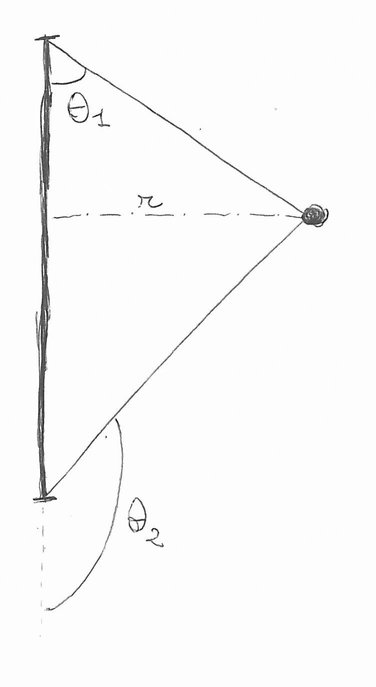
\includegraphics[width=0.95\linewidth]{SegmentoFilo}
    \end{center}
  \end{minipage}%
  \begin{minipage}{0.5\linewidth}
    Il campo magnetico in un qualunque punto dello spazio è dato da
    \begin{equation*}
      \vec B = \hat\varphi \frac{\mu_0 I}{4 \pi r} \int_{\theta_1}^{\theta_2} \sin \theta \de \theta
    \end{equation*}
    dove $\theta_1$ e $\theta_2$ sono l'angolo iniziale e l'angolo finale
    che la congiungente al filo forma con il filo stesso.
  \end{minipage}
}

\formula{Filo infinito}{
  Un filo lungo l'asse $\hat z$ percorso da corrente $I$ genera
  \begin{equation*}
    \vec B(\vec r)=\hat\varphi \frac{\muz I}{2\pi\rho}
  \end{equation*}
  dove $\hat\varphi$ è orientato in modo che se il pollice della mano destra è $\hat z$, le restanti dita ne descrivono il verso.
}

\formula{Solenoide cilindrico}{
  Un solenoide di raggio $a$, con $n$ spire per unità di lunghezza percorse da corrente $I$, disposto lungo l'asse $\hat z$ genera
  \begin{equation*}
    \vec B(\vec r)=\hat z\muz nI
  \end{equation*}
  che è diretto in modo che se le dita della mano destra seguono $I$,
  allora il pollice detta il verso di $\vec B$.

  Inoltre, la sua autoinduttanza vale $L = \mu_0 \frac{N^2 a^2 \pi}{l}$,
  con $l$ la sua lunghezza, $N$ il numero di spire totali
  ($n = \frac{N}{l}$)
}

\formula{Spira}{
  Una spira di raggio $a$ percorsa da corrente $I$ con asse lungo $\hat z$, genera sull'asse $\hat z$
  \begin{equation*}
    \vec B(z)=\hat z\frac{\muz a^2I}{2\left(z^2+a^2\right)^{\frac 32}}
  \end{equation*}
  dove anche questa volta $\vec B$ è il pollice della mano destra e le altre dita seguono $I$.
}

\section{Elettrodinamica}
Ora tratteremo i casi, finora non considerati, di campo elettrico non costante e come questo incida sul campo magnetico.
Questo farà sì che il campo elettrico non sia più conservativo e perciò non esista più un potenziale.

\formula{Conduttore}{
  Per conduttore ora si intenderà che la forza di Lorentz è nulla al suo
  interno.
}

\formula{II equazione di Maxwell}{
  \begin{equation*}
    \rot\vec E=-\frac{\partial \vec B}{\partial t}
  \end{equation*}
}

\formula{Legge di Lenz}{
  Nel caso di un circuito, la forma integrale della II equazione di Maxwell diventa:
  \begin{equation*}
    \mathcal E=-\frac \de{\de t}\int_S \vec B\dotp\de\vec S=-\frac {\de\Phi_B}{\de t}
  \end{equation*}
  dove $\mathcal E$ è la forza elettromotrice (f.e.m.) indotta sul circuito e $\Phi_B$ è il flusso di campo magnetico attraverso la superficie racchiusa dal circuito.
  Il segno della f.e.m. indotta è tale da opporsi sempre alla variazione di corrente.
}

\formula{IV equazione di Maxwell}{
  Questa legge generalizza sia l'equazione di continuità sia la legge di Ampère al caso elettrodinamico:
  \begin{equation*}
    \frac 1{c^2}\frac{\partial \vec E}{\partial t}-\rot\vec B+\muz\vec J=0
  \end{equation*}
}

\formula{Circuito RLC}{
  \begin{equation*}
    \ddot{Q} + \frac{R}{L} \dot{Q} + \frac{1}{LC} Q = 0
  \end{equation*}

  Sono quindi esponenziali smorzati con
  $$\alpha_{1,2} = \frac{- R \pm \sqrt{R^2 - 4 \frac{L}{C}}}{2 L}$$
}

\section{Formule di M. Complete}
\begin{equation*}
  \div {\vec E} = \frac{\rho}{\epsilon_0}
\end{equation*}
\begin{equation*}
  \div {\vec B} = 0
\end{equation*}
\begin{equation*}
  \rot {\vec E} = - \dep{\vec B}{t}
\end{equation*}
\begin{equation*}
  \rot {\vec B} = \epsilon_0 \mu_0 \dep{\vec E}{t} + \mu_0 \vec J
\end{equation*}

\section{Induzione magnetica}

\formula{Induttanza}{
  L'induttanza è una costante $L$ dipendente dalla geometria del circuito, tale che
  \begin{equation*}
    \Phi_B=LI
  \end{equation*}
  dove $\Phi_B$ è il flusso di campo magnetico generato dal circuito stesso.
}

\formula{Induttore}{
  Un induttore è una componente di un circuito la cui induttanza non è trascurabile. L'esempio tipico è un solenoide.
}

\formula{Mutua induzione}{
  Chiamando $\vec{\mathcal E}$ il vettore delle f.e.m. indotte e $\vec I$ il vettore delle correnti di $n$ circuiti, esiste una matrice $L$ simmetrica, che sulla diagonale ha le autoinduttanze dei singoli circuiti, tale che:
  \begin{equation*}
    \vec {\mathcal E}=-L\frac{\de \vec I}{\de t}
  \end{equation*}
  e il valore $L_{ij}=L_{ji}$ si calcola con
  \begin{equation*}
    L_{ij}=L_{ji}=\frac {\muz}{4\pi}\oint_{\gamma_i}\oint_{\gamma_j}\frac{\de \vec l_i\dotp\de\vec l_j}{r}
  \end{equation*}
  dove con $r$ indichiamo la distanza tra i punti in cui stiamo integrando.
}

\formula{Mutua induzione tra due circuiti}{
  \begin{center}
    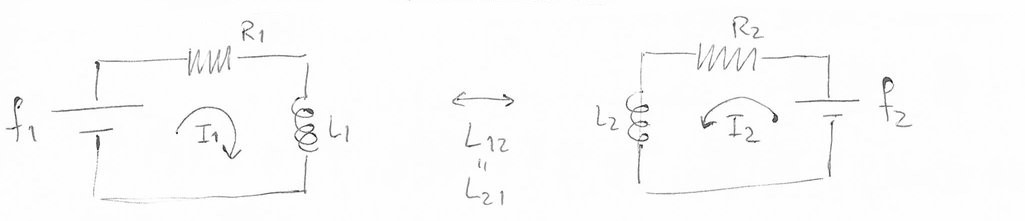
\includegraphics[width=0.9\linewidth]{MutuaInduzioneCircuiti}
  \end{center}
    
  Nel caso di due circuiti come in figura con mutua induzione tra di
  essi si hanno le seguenti formule:

  \begin{eqsystem}{c}
    f_1 = I_1 R_1 + L_1 \dot{I_1} + L_{12} \dot{I_2} \\
    f_2 = I_2 R_2 + L_2 \dot{I_2} + L_{21} \dot{I_1} \\
  \end{eqsystem}
}

\formula{Energia di un induttore}{
  \begin{equation*}
    U=\frac 12LI^2
  \end{equation*}
  e nel caso di un sistema di induttori:
  \begin{equation*}
    U=\frac 12 \vec I^{\,T}L\vec I
  \end{equation*}
}

\formula{Circuiti RLC}{
  \begin{equation*}
    \mathcal E=RI+\frac QC + L\frac{\de I}{\de t}=\frac QC+R\frac{\de Q}{\de t}+L\frac{\de^2Q}{\de t^2}
  \end{equation*}
}

\section{Alcune induttanze}
\formula{Induttanza cavo coassiale}{
  \begin{center}
    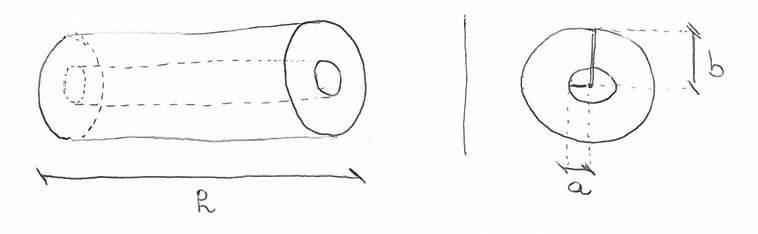
\includegraphics[width=0.9\linewidth]{CavoCoassiale}
  \end{center}
    
  dove supponiamo che $b > a$, $h >> b \simeq a$. Allora l'induttanza è
  data da $L = \frac{\mu_0 h}{2 \pi} \log(\frac{b}{a})$
}

\section{Formule nei materiali}
\formula{Formula fondamentale}{
  $$\vec{D} = \epsilon_0 \epsilon_r \vec{E} = \epsilon_0 \vec{E} + \vec{P}$$
  $\vec P$ viene chiamata densità di dipolo
}

\formula{Densità di carica}{
  $$\rho_\text{TOT} = \rho_\text{EXT} + \rho_\text{IND}$$
  $$\div{\vec P} = - \rho_\text{IND}$$
  $$\div{\vec D} = \rho_\text{EXT}$$
  $$\vec{P} \cdot \hat{n} = \sigma_\text{IND}$$
}

\formula{Condizioni superficiali campi elettrici}{
  \begin{minipage}{0.35\linewidth}
    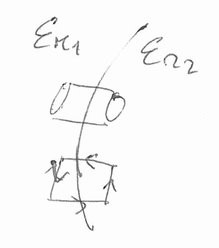
\includegraphics[width=0.95\linewidth]{SaltiCampiElettrici}
  \end{minipage}%
  \begin{minipage}{0.6\linewidth}
    Come si relazionano i salti dei campi nel passare da una parte della
    superficie all'altra?

    \begin{eqsystem}{c}
      \vec{D_{\bot_1}} - \vec{D_{\bot_2}} = \sigma_\text{EXT} \\
      \vec{E_{\parl_1}} = \vec{E_{\parl_2}}                   \\
    \end{eqsystem}
  \end{minipage}
}

\formula{Energia elettrica in presenza di dielettrici}{
  $$U = \frac{1}{2} \int \vec{D} \dotp \vec{E}$$

  E la densità di energia è
  $u = \frac{{\vec D}^2}{2 \epsilon_0 \epsilon_r}$
}

\formula{Campi magnetici nella materia}{
  $\vec \mu$ è la densità di momento magnetico
  
  \begin{displaymath}
    \begin{array}{cr}
      \vec{J_\IND} = \rot {\vec \mu}            &                       \\
      \vec{k_\IND} = {\vec \mu} \times {\hat n} & \text{(superficiale)} \\
    \end{array}
  \end{displaymath}

  Se inoltre definiamo $\vec H = \frac{\vec B}{\mu_0} - {\vec \mu} =
  \frac{1}{\mu_0} (1 - \chi_m) {\vec B}$ valgono le equazioni:
  \begin{displaymath}
    \begin{array}{c}
      \rot {\vec H} = {\vec J_\EXT} \\
      \div {\vec B} = 0             \\
    \end{array}
  \end{displaymath}

  $$\frac{1}{\mu_0 \mu_r} = \frac{1}{\mu_0} (1 - \chi_m)$$
  $$\vec H = \frac{1}{\mu_0 \mu_r} {\vec B}$$
}

\formula{Condizioni superficiali campo magnetico}{
  \begin{minipage}{0.35\linewidth}
    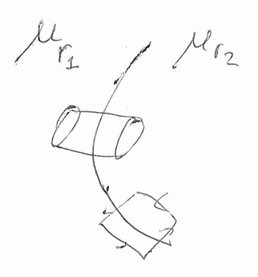
\includegraphics[width=0.95\linewidth]{SaltiCampiMagnetici}
  \end{minipage}%
  \begin{minipage}{0.6\linewidth}
    Come si relazionano i salti dei campi nel passare da una parte della
    superficie all'altra?

    \begin{eqsystem}{c}
      \vec{B_{\bot_1}} = \vec{B_{\bot_2}} \\
      \vec{H_{\parl_1}} - \vec{H_{\parl_2}} = \vec{k_\EXT} \\
    \end{eqsystem}
  \end{minipage}
}


\section{Esempi particolari}
\formula{Sfera uniformemente polarizzata}{
  Il problema è dato in termini della densità di dipolo:
  \begin{eqsystem}{cr}
    \vec P = p \hat{z} & \text{se } r \le a \\
    \vec P = 0         & \text{se } r > a   \\
  \end{eqsystem}

  Allora, se non c'è $\rho_\text{EXT}$, si ha $\rho_\text{IND} = 0$,
  $\sigma_\text{IND} = \vec P \dotp \hat{n} = p \cos \theta$, con
  $r = a$.

  Il campo è
  \begin{eqsystem}{rl}
    \vec E (r < a) = & \frac{p}{3 \epsilon_0} \hat{z} \\
    \vec E (r > a) = & \frac{\vec{P_\text{TOT}} \dotp \vec{r}}{4 \pi \epsilon_0 r^2} \\
  \end{eqsystem}
  dove $\vec{P_\text{TOT}} = \frac{4}{3} \pi a^3 p \hat{z}$
}

\section{Onde Elettromagnetiche}
\formula{Equazioni nel vuoto}{
  Definiamo
  $\square = \nabla^2 - \frac{1}{c^2} \frac{\partial^2}{\partial t^2}$

  Allora le equazioni nel vuoto diventano $\square {\vec B} = 0$ e
  $\square {\vec E} = 0$.
}

\formula{Formula Onda Piana nel vuoto}{
  Un'onda piana nel vuoto ha la seguente forma:
  \begin{eqsystem}{rl}
    \vec E = & \vec{E_0} \cos (\vec{k} \dotp \vec{r} - \omega t + \varphi_0) \\
    \vec B = & \vec{B_0} \cos (\vec{K} \dotp \vec{r} - \omega t + \varphi_0) \\
  \end{eqsystem}
  con $\vec{B_0} = \frac{1}{c} \hat{k} \times \vec{E}$ e $\omega = ck$.
  Esse hanno polarizzazione lineare.

  Abbiamo invece anche quelle con polarizzazione circolare:
  \begin{eqsystem}{rl}
    \vec E = & (\vec{a_0} \pm i \hat{k} \times \vec{a_0}) e^{i (\vec{k} \dotp \vec{r} - \omega t + \varphi_0)}             \\
    \vec B = & \frac{1}{c} (\hat{k} \times \vec{a_0} \mp i \vec{a_0}) e^{i (\vec{k} \dotp \vec{r} - \omega t + \varphi_0)} \\
  \end{eqsystem}

  Chiamiamo vettore di Poynting
  $\vec{I} = \frac{1}{\mu_0} (\vec{E} \times \vec{B})$, siccome si ha,
  fissato un volume $V$, e detta $\Sigma = \partial V$ il suo bordo:
  $$\frac{\de}{\de t} \lrt{\int_{V_\epsilon} u_E + u_B} = -
  \frac{1}{\mu_0} \int_\Sigma (\vec{E} \times \vec{B}) \dotp \de{\vec{s}}$$

  E la densità di quantità di moto $\vec P = \frac{1}{c} \vec S$. Densità di momento angolare $\vec{m_\Omega} = (\vec r - \vec \Omega) \times \vec{P}(\vec r)$
}

\formula{Riflessione di un onda}{
  $\vec E = \vec{E_+} + \vec{E_-}$ ed
  anche $\vec B = \vec{B_+} + \vec{B_-}$, dove con il $+$ indichiamo i
  campi incidenti e con il $-$ indichiamo i campi riflessi.

  % TODO: Da finire

  Ricordiamo che per le onde piane si ha $\vec{\nabla} = i \vec{k}$, ovvero $\rot (e^{\vec k \cdot \vec r} \vec u) = (i \vec{k} \times u) e^{\vec k \cdot \vec r}$ e simili.
}

\formula{Dipolo oscillante}{
}

\formula{Velocità della luce in un mezzo}{
  $v = \frac{c}{\sqrt{\epsilon_r \mu_r}}$ è la velocità della luce.

  Inoltre $n_r = \frac{v}{c}$ si dice indice di rifrazione
}

\formula{Onde incidenti, rifratte, riflesse}{
  \begin{center}
    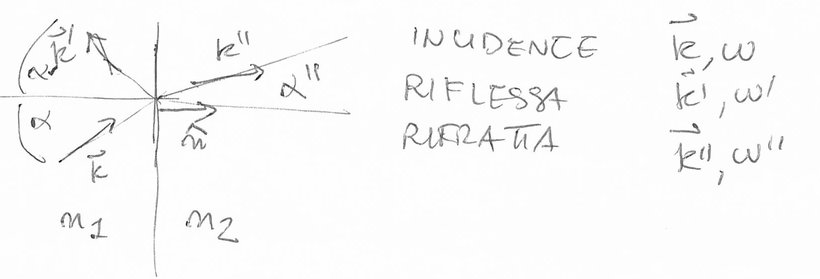
\includegraphics[width=0.95\linewidth]{OndeRiflesseRifratte}
  \end{center}

  Imponendo la continuità dei campi nei materiali si ottiene $\omega =
  \omega' = \omega''$, $\alpha = \alpha'$, ovvero che l'angolo di
  riflessione è uguale all'angolo di incidenza.

  Inoltre per la relazione di snell
  $n_2 \sin \alpha'' = n_1 \sin \alpha$

  Se la polarizzazione è ortogonale sia a $\hat{k}$ sia a $\hat{n}$,
  vale che
  \begin{displaymath}
    \begin{array}{c}
      E_0' = \frac{n_1 \cos \alpha - n_2 \cos \alpha'}{n_1 \cos \alpha + n_2 \cos \alpha''} \\
      E_0'' = E_0 \frac{2 n_1 \cos \alpha}{n_1 \cos \alpha + n_2 \cos \alpha'}              \\
    \end{array}
  \end{displaymath}
}

\formula{Potenziali ritardati}{
  \begin{eqsystem}{rl}
    V =       & \frac{1}{4 \pi \epsilon_0} \int \frac{\rho(\vec{r}', t - \frac{\abs{\vec{r} - \vec{r}'}}{c})}{\abs{\vec{r} - \vec{r}'}} \de^3 r' \\
    \vec{A} = & \frac{\mu_0}{4 \pi} \int \frac{\vec{J}(\vec{r}', t - \frac{\abs{\vec{r} - \vec{r}'}}{c})}{\abs{\vec{r} - \vec{r}'}} \de^3 r'     \\
  \end{eqsystem}
  Ed è soddisfatta la Gauge di Lorentz: $\div {\vec A} + \frac{1}{c^2}
  \frac{\partial^2 V}{\partial t^2} = 0$.
}


\section{Integrali ``Noti''}
\begin{equation*}
  \int \frac{r \de r}{(r^2+1)^{\frac{3}{2}}} = - \frac{1}{\sqrt{r^2 + 1}}
\end{equation*}

\begin{equation*}
  \int e^{\alpha t} \de t = \frac{1}{\alpha} e^{\alpha t}
\end{equation*}

\begin{equation*}
  \int t e^{\alpha t} \de t = \frac{\alpha t - 1}{\alpha^2} e^{\alpha t}
\end{equation*}

\section{Operatori differenziali}

  \formula{Gradiente in cartesiane}
  \begin{equation*}
    \grad f = \dep{f}{x} \hat{x} +
    \dep{f}{y} \hat{y} +
    \dep{f}{z} \hat{z}
  \end{equation*}
  
  \formula{Gradiente in cilindriche}
  \begin{equation*}
    \grad f = \dep{f}{\rho} \hat{\rho} +
    \frac{1}{\rho} \dep{f}{\phi} \hat{\phi} +
    \dep{f}{z} \hat{z}
  \end{equation*}
  
  \formula{Gradiente in sferiche}
  \begin{equation*}
    \grad f = \dep{f}{r} \hat{r} +
    \frac{1}{r} \dep{f}{\theta} \hat{\theta} +
    \frac{1}{r \sin \theta} \dep{f}{\phi} \hat{\phi}
  \end{equation*}
  
  \formula{Divergenza in cartesiane}
  \begin{equation*}
    \div A = \dep{A_x}{x} + \dep{A_y}{y} + \dep{A_z}{z}
  \end{equation*}
  
  \formula{Divergenza in cilindriche}
  \begin{equation*}
    \div A = \frac{1}{\rho} \dep{(\rho A_\rho)}{\rho} +
    \frac{1}{\rho} \dep{A_\phi}{\phi} +
    \dep{A_z}{z}
  \end{equation*}
  
  \formula{Divergenza in sferiche}
  \begin{equation*}
    \div A = \frac{1}{r^2} \dep{(r^2 A_r)}{r} +
    \frac{1}{r \sin \theta} \dep{(A_\theta \sin\theta)}{\theta} +
    \frac{1}{r \sin\theta} \dep{A_\phi}{\phi}
  \end{equation*}

\formula{Rotore in cartesiane}
\begin{align*}
  \rot A = \lrb{\dep{A_z}{y} - \dep{A_y}{z}} \hat{x} + \\
  \lrb{\dep{A_x}{z} - \dep{A_z}{x}} \hat{y} + \\
  \lrb{\dep{A_y}{x} - \dep{A_x}{y}} \hat{z}
\end{align*}

\formula{Rotore in cilindriche}
\begin{align*}
  \rot A = \lrb{\frac{1}{\rho} \dep{A_z}{\phi} - \dep{A_\phi}{z}} \hat{\rho} + \\
  \lrb{\dep{A_\rho}{z} - \dep{A_z}{\rho}} \hat{\phi} + \\
  \frac{1}{\rho} \lrb{\dep{(\rho A_\phi)}{\rho} - \dep{A_\rho}{\phi}} \hat{z}
\end{align*}

\formula{Rotore in sferiche}
\begin{align*}
  \rot A = \frac{1}{r \sin\theta} \lrb{\dep{(A_\phi \sin\theta)}{\phi} - \dep{A_\theta}{\phi}} \hat{r} + \\
  \frac{1}{r} \lrb{\frac{1}{\sin\theta} \dep{A_r}{\phi} - \dep{(r A_\phi)}{r}} \hat{\theta} + \\
  \frac{1}{r} \lrb{\dep{(r A_\theta)}{r} - \dep{A_r}{\theta}} \hat{\phi}
\end{align*}
\end{multicols}
\end{document}

% TODO: Scrivere anche i cambi per i sistemi di coordinate polari
% cartesiane e cilindriche.

